%%%%%%%%%%%%%%%%%%%%%%%%%%%%%%%%%%%%%%%%%
% Programming/Coding Assignment
% LaTeX Template
%
% This template has been downloaded from:
% http://www.latextemplates.com
%
% Original author:
% Ted Pavlic (http://www.tedpavlic.com)
%
% Note:
% The \lipsum[#] commands throughout this template generate dummy text
% to fill the template out. These commands should all be removed when 
% writing assignment content.
%
% This template uses a Perl script as an example snippet of code, most other
% languages are also usable. Configure them in the "CODE INCLUSION 
% CONFIGURATION" section.
%
%%%%%%%%%%%%%%%%%%%%%%%%%%%%%%%%%%%%%%%%%

%----------------------------------------------------------------------------------------
%	PACKAGES AND OTHER DOCUMENT CONFIGURATIONS
%----------------------------------------------------------------------------------------

\documentclass{article}

\usepackage{fancyhdr} % Required for custom headers
\usepackage{lastpage} % Required to determine the last page for the footer
\usepackage{extramarks} % Required for headers and footers
\usepackage[usenames,dvipsnames]{color} % Required for custom colors
\usepackage{graphicx} % Required to insert images
\usepackage{subcaption}
\usepackage{listings} % Required for insertion of code
\usepackage{courier} % Required for the courier font
\usepackage{lipsum} % Used for inserting dummy 'Lorem ipsum' text into the template
\usepackage{amsmath}
\usepackage{amssymb}
\usepackage{amsthm}


% Margins
\topmargin=-0.45in
\evensidemargin=0in
\oddsidemargin=0in
\textwidth=6.5in
\textheight=9.0in
\headsep=0.25in

\linespread{1.1} % Line spacing

% Set up the header and footer
\pagestyle{fancy}
\lhead{\hmwkAuthorName} % Top left header
\chead{\hmwkClass\ (\hmwkClassTime): \hmwkTitle} % Top center head
%\rhead{\firstxmark} % Top right header
\lfoot{\lastxmark} % Bottom left footer
\cfoot{} % Bottom center footer
\rfoot{Page\ \thepage\ of\ \protect\pageref{LastPage}} % Bottom right footer
\renewcommand\headrulewidth{0.4pt} % Size of the header rule
\renewcommand\footrulewidth{0.4pt} % Size of the footer rule

\setlength\parindent{0pt} % Removes all indentation from paragraphs

%----------------------------------------------------------------------------------------
%	CODE INCLUSION CONFIGURATION
%----------------------------------------------------------------------------------------

\definecolor{MyDarkGreen}{rgb}{0.0,0.4,0.0} % This is the color used for comments
\lstloadlanguages{Perl} % Load Perl syntax for listings, for a list of other languages supported see: ftp://ftp.tex.ac.uk/tex-archive/macros/latex/contrib/listings/listings.pdf
\lstset{language=Perl, % Use Perl in this example
        frame=single, % Single frame around code
        basicstyle=\small\ttfamily, % Use small true type font
        keywordstyle=[1]\color{Blue}\bf, % Perl functions bold and blue
        keywordstyle=[2]\color{Purple}, % Perl function arguments purple
        keywordstyle=[3]\color{Blue}\underbar, % Custom functions underlined and blue
        identifierstyle=, % Nothing special about identifiers                                         
        commentstyle=\usefont{T1}{pcr}{m}{sl}\color{MyDarkGreen}\small, % Comments small dark green courier font
        stringstyle=\color{Purple}, % Strings are purple
        showstringspaces=false, % Don't put marks in string spaces
        tabsize=5, % 5 spaces per tab
        %
        % Put standard Perl functions not included in the default language here
        morekeywords={rand},
        %
        % Put Perl function parameters here
        morekeywords=[2]{on, off, interp},
        %
        % Put user defined functions here
        morekeywords=[3]{test},
       	%
        morecomment=[l][\color{Blue}]{...}, % Line continuation (...) like blue comment
        numbers=left, % Line numbers on left
        firstnumber=1, % Line numbers start with line 1
        numberstyle=\tiny\color{Blue}, % Line numbers are blue and small
        stepnumber=5 % Line numbers go in steps of 5
}

% Creates a new command to include a perl script, the first parameter is the filename of the script (without .pl), the second parameter is the caption
\newcommand{\perlscript}[2]{
\begin{itemize}
\item[]\lstinputlisting[caption=#2,label=#1]{#1.pl}
\end{itemize}
}

%----------------------------------------------------------------------------------------
%	DOCUMENT STRUCTURE COMMANDS
%	Skip this unless you know what you're doing
%----------------------------------------------------------------------------------------

% Header and footer for when a page split occurs within a problem environment
\newcommand{\enterProblemHeader}[1]{
%\nobreak\extramarks{#1}{#1 continued on next page\ldots}\nobreak
%\nobreak\extramarks{#1 (continued)}{#1 continued on next page\ldots}\nobreak
}

% Header and footer for when a page split occurs between problem environments
\newcommand{\exitProblemHeader}[1]{
%\nobreak\extramarks{#1 (continued)}{#1 continued on next page\ldots}\nobreak
%\nobreak\extramarks{#1}{}\nobreak
}

\setcounter{secnumdepth}{0} % Removes default section numbers
\newcounter{homeworkProblemCounter} % Creates a counter to keep track of the number of problems
\setcounter{homeworkProblemCounter}{0}

\newcommand{\homeworkProblemName}{}
\newenvironment{homeworkProblem}[1][Part \arabic{homeworkProblemCounter}]{ % Makes a new environment called homeworkProblem which takes 1 argument (custom name) but the default is "Problem #"
\stepcounter{homeworkProblemCounter} % Increase counter for number of problems
\renewcommand{\homeworkProblemName}{#1} % Assign \homeworkProblemName the name of the problem
\section{\homeworkProblemName} % Make a section in the document with the custom problem count
\enterProblemHeader{\homeworkProblemName} % Header and footer within the environment
}{
\exitProblemHeader{\homeworkProblemName} % Header and footer after the environment
}

\newcommand{\problemAnswer}[1]{ % Defines the problem answer command with the content as the only argument
\noindent\framebox[\columnwidth][c]{\begin{minipage}{0.98\columnwidth}#1\end{minipage}} % Makes the box around the problem answer and puts the content inside
}

\newcommand{\homeworkSectionName}{}
\newenvironment{homeworkSection}[1]{ % New environment for sections within homework problems, takes 1 argument - the name of the section
\renewcommand{\homeworkSectionName}{#1} % Assign \homeworkSectionName to the name of the section from the environment argument
\subsection{\homeworkSectionName} % Make a subsection with the custom name of the subsection
\enterProblemHeader{\homeworkProblemName\ [\homeworkSectionName]} % Header and footer within the environment
}{
\enterProblemHeader{\homeworkProblemName} % Header and footer after the environment
}

%----------------------------------------------------------------------------------------
%	NAME AND CLASS SECTION
%----------------------------------------------------------------------------------------

\newcommand{\hmwkTitle}{Assignment\ \#$1$} % Assignment title
\newcommand{\hmwkDueDate}{Monday,\ January\ 29,\ 2018} % Due date
\newcommand{\hmwkClass}{CSC411} % Course/class
\newcommand{\hmwkClassTime}{L0101} % Class/lecture time
\newcommand{\hmwkAuthorName}{Yifei Dong} % Your name

%----------------------------------------------------------------------------------------
%	TITLE PAGE
%----------------------------------------------------------------------------------------

\title{
\vspace{2in}
\textmd{\textbf{\hmwkClass:\ \hmwkTitle}}\\
\normalsize\vspace{0.1in}\small{Due\ on\ \hmwkDueDate}\\
\vspace{0.1in}
\vspace{3in}
}

\author{\textbf{\hmwkAuthorName}}
\date{} % Insert date here if you want it to appear below your name

%----------------------------------------------------------------------------------------

\begin{document}

\maketitle
\clearpage
%----------------------------------------------------------------------------------------
%	PROBLEM 1
%----------------------------------------------------------------------------------------

% To have just one problem per page, simply put a \clearpage after each problem

\begin{homeworkProblem}

\noindent \textit{Dataset description}

The original images are from a subset of FaceScrub dataset. The images are cropped by the provided dimensions and converted into grayscale. The final dataset consists of $5400$ grayscale $32\times 32$-pixel of images of 6 actor and actresses, each of them with 90 images. The uncropped images are saved in a folder called uncropped and the cropped images are saved in a folder called cropped. Samples of uncropped and cropped images are shown in Figure 1.


\begin{figure*}[!ht]
\begin{subfigure}{.35\textwidth}
  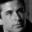
\includegraphics[width=.5\linewidth]{baldwin10.jpg}
  \caption{Uncropped Baldwin1}
  \label{fig:sfig1}
\end{subfigure}
\begin{subfigure}{.35\textwidth}
  
\includegraphics[width=.5\linewidth]{baldwin34.jpg}
  \caption{Uncropped Baldwin2}
  \label{fig:sfig2}
\end{subfigure}%
\begin{subfigure}{.35\textwidth}
  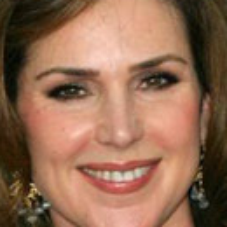
\includegraphics[width=.5\linewidth]{gilpin65.jpg}
  \caption{Uncropped Gilpin}
  \label{fig:sfig3}
\end{subfigure}
\begin{subfigure}{.35\textwidth}
  \includegraphics[width=.5\linewidth]{baldwin10_cro.jpg}
  \caption{Cropped Baldwin1}
  \label{fig:sfig4}
\end{subfigure}%
\begin{subfigure}{.35\textwidth}
  \includegraphics[width=.5\linewidth]{baldwin34_cro.jpg}
  \caption{Cropped Baldwin2}
  \label{fig:sfig5}
\end{subfigure}
\begin{subfigure}{.35\textwidth}
  \includegraphics[width=.5\linewidth]{gilpin65_pro.jpg}
  \caption{Cropped Gilpin}
  \label{fig:sfig6}%
\end{subfigure}
\caption{}
\label{fig:pcs}
\end{figure*}

From the samples above, we could see that the faces are cropped correctly. From the two images of Baldwin, the similarity of the two iamges can be seen by comparing the eyes, nose and mouth. And by comparing the cropped image of Baldwin to the cropped image of Gilpin we can see that both of them have only the face cropped. So the images can be compared between actor and actresses as well.\\

However, there are some issues of cropped images. Some examples are shown below in Figure 2. The first issue I faced is that some images are not correct images of the person, so the cropped image is something random. Another issue is that although the face is in the cropped image but the face is not shown properly. A third issue is that some original images are not downloaded properly so the images could not be read and thus cannot be cropped.

\begin{figure*}[!ht]
\begin{subfigure}{.5\textwidth}
  
\includegraphics[width=.5\linewidth]{baldwin67.jpg}
  \caption{Uncropped Baldwin}
  \label{fig:a2.1}
\end{subfigure}%
\begin{subfigure}{.35\textwidth}
  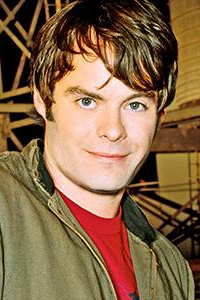
\includegraphics[width=.5\linewidth]{hader98.jpg}
  \caption{Uncropped Harmon}
  \label{fig:a2.2}
\end{subfigure}%


\begin{subfigure}{.5\textwidth}
  \includegraphics[width=.5\linewidth]{baldwin67_cro.jpg}
  \caption{Cropped Baldwin }
  \label{fig:a2.3}
\end{subfigure}%
\begin{subfigure}{.5\textwidth}
  \includegraphics[width=.5\linewidth]{hader98_cro.jpg}
  \caption{Cropped Harmon}
  \label{fig:a2.4}
\end{subfigure}%

\caption{}
\label{fig:part1}
\end{figure*}

\end{homeworkProblem}
\clearpage
%----------------------------------------------------------------------------------------
%	PROBLEM 2
%----------------------------------------------------------------------------------------

\begin{homeworkProblem}
\noindent \textit{Separate the dataset into three non-overlapping parts}\\
The cropped grayscale faces are separated into three non-overlapping parts, which are training set, validation set and test set. I put all the cropped images into one folder called cropped but build three separate dictionaries for each set. The dictionaries are called tra, val and tes. I used the name of the images as the keys of dictionaries. For each key, there are two parameters. The first is the name of the actor or actress, the second is the gender. If it's an actor, the second parameter will be "M", otherwise it will be "F".\\

For example, a dictionary containing two images would look like this:
\begin{verbatim}
    dict = {'bracco72.jpg': ['bracco', 'F'], 'baldwin79.jpg': ['baldwin', 'M']}
\end{verbatim}

The dictionaries are built while saving the images. When a cropped image is successfully saved, it will be added to the corresponding dictionary.\\

I first built three empty dictionaries call tra, val and tes. Images are read and saved in the order of the act list, which contains the names of the actor and actresses we want. The outer for loop read and saved images of a single person each iteration. Therefore, in the inner for loop, I recorded the number of saved cropped images. When the number is smaller than 70, I save the images to tra dictionary. When the number is between 70 and 80, I save the images to val dictionary. When the number is between 80 and 90, I save the iamges to the tes dictionary. Thus, the three non-overlapping parts are created. 



\end{homeworkProblem}
\clearpage
%----------------------------------------------------------------------------------------
%	PROBLEM 3
%----------------------------------------------------------------------------------------

\begin{homeworkProblem}
\noindent \textit{Use Linear Regression in order to build a classifier to distinguish pictures of Alec Baldwin form pictures of Steve Carell.}\\
The cost function I minimized is:
\[J(\theta_0,\theta_1,...,\theta_{1024})= \sum_{i=1}^{140} \left( h_{\theta}(x^{(i)})-y^{(i)}\right)^2\]
\includegraphics[scale = 0.7]{part3a.png}\\
The theta is of size $(1025, 1)$ since there are $32 \times 32 = 1024$ pixels per image and $\theta_0$ is added as the intercept of Linear regression.\(( h_{\theta}(x^{(i)})-y^{(i)})^2\) is added $140$ times because there are 140 images.\\

The value of the cost function on training set is $f_{min}(x) = 0.69$. The value of the cost function on validation set id $f_{min}(x) = 0.04$.\\

The accuracy of the Part 3 classifier on training set is $100\%$.
The accuracy of the Part 3 classifier on validation set is $90\%$.\\

\includegraphics[scale = 0.7]{part3}\\
The above is the code I used to compute the output of the classifier. Theta was computed by the classifier called classifierBC. And the result y is compute by the formula $y = \theta^{T}x$, where x is matrix of flattened image.\\

There are a few things I did in order to get the system to work.\\
1. The threshold $\epsilon$ in Gradient Descent function could change the behaviour of the system, as well as the maximum number of iterations. When the threshold is too high and the max\_iter is too low, the gradient descent function would stop before the minimum value of cost function is found.\\
2. When $\alpha$ was set too large or too small. The minimum is passed and the gradient descent function diverged. I first set $\alpha = 10^{-8}$ and the gradient descent function stopped almost immediately. I finally set $\alpha$ to $0.00001$ after a few times of testing.\\
3. I set the initial theta as an array of size $(1025, 1)$ with the same value. When I set the initial theta value as an array of 0s. The accuracy of training set is $100\%$ as well as the test set. But the accuracy for validation set is only $85\%$. This might be overfitting. I tried with a few theta values. When the initial theta is set to 0.3, the accuracy is $100\%$ for training set, $90\%$ for validation set, and $95\%$ for test set.\\


\end{homeworkProblem}
\clearpage

%----------------------------------------------------------------------------------------
%	PROBLEM 4
%----------------------------------------------------------------------------------------

\begin{homeworkProblem}

a)\\

\begin{figure*}[!ht]
\begin{subfigure}{.55\textwidth}
  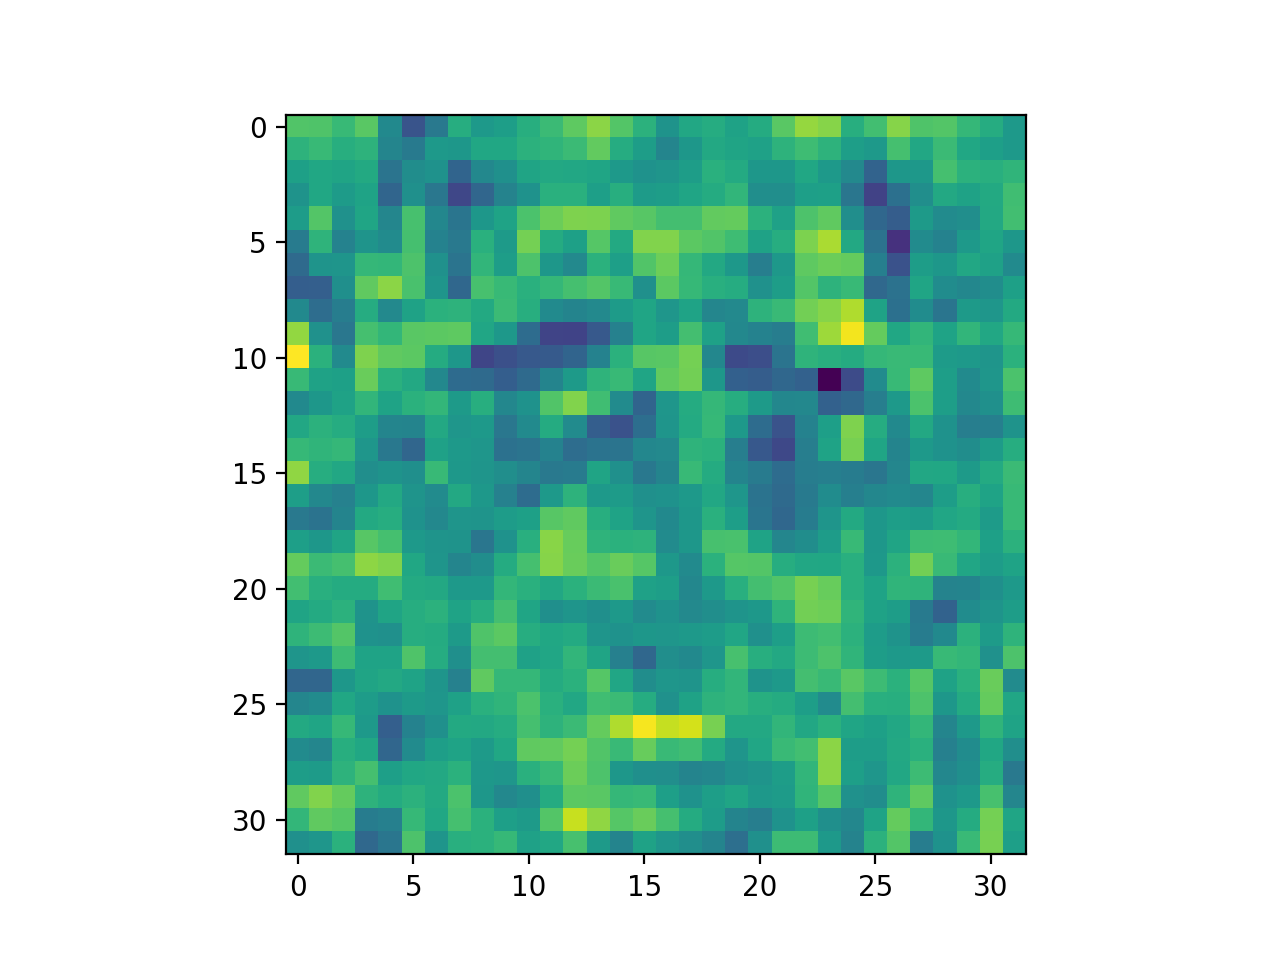
\includegraphics[width=.8\linewidth]{part4a1}
  \caption{$\theta$ got from full training set}
  \label{fig:4a1}
\end{subfigure}%
\begin{subfigure}{.55\textwidth}
  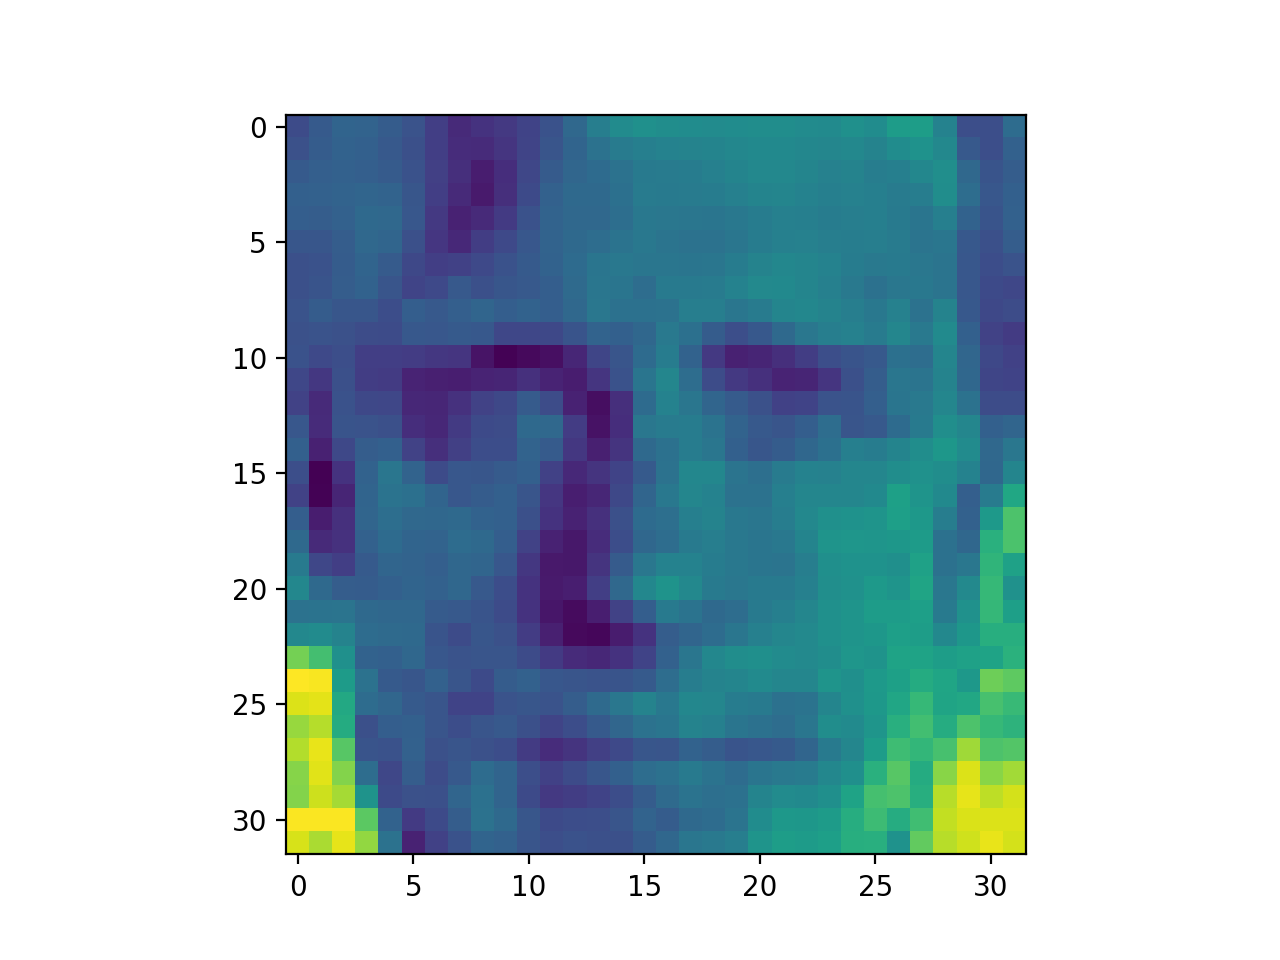
\includegraphics[width=.8\linewidth]{part4a2.png}
  \caption{$\theta$ got from a training set with two images}
  \label{fig:4a2}
\end{subfigure}%

\caption{}
\label{fig:part4}
\end{figure*}

b)\\
\begin{figure*}[!ht]
\begin{subfigure}{.55\textwidth}
  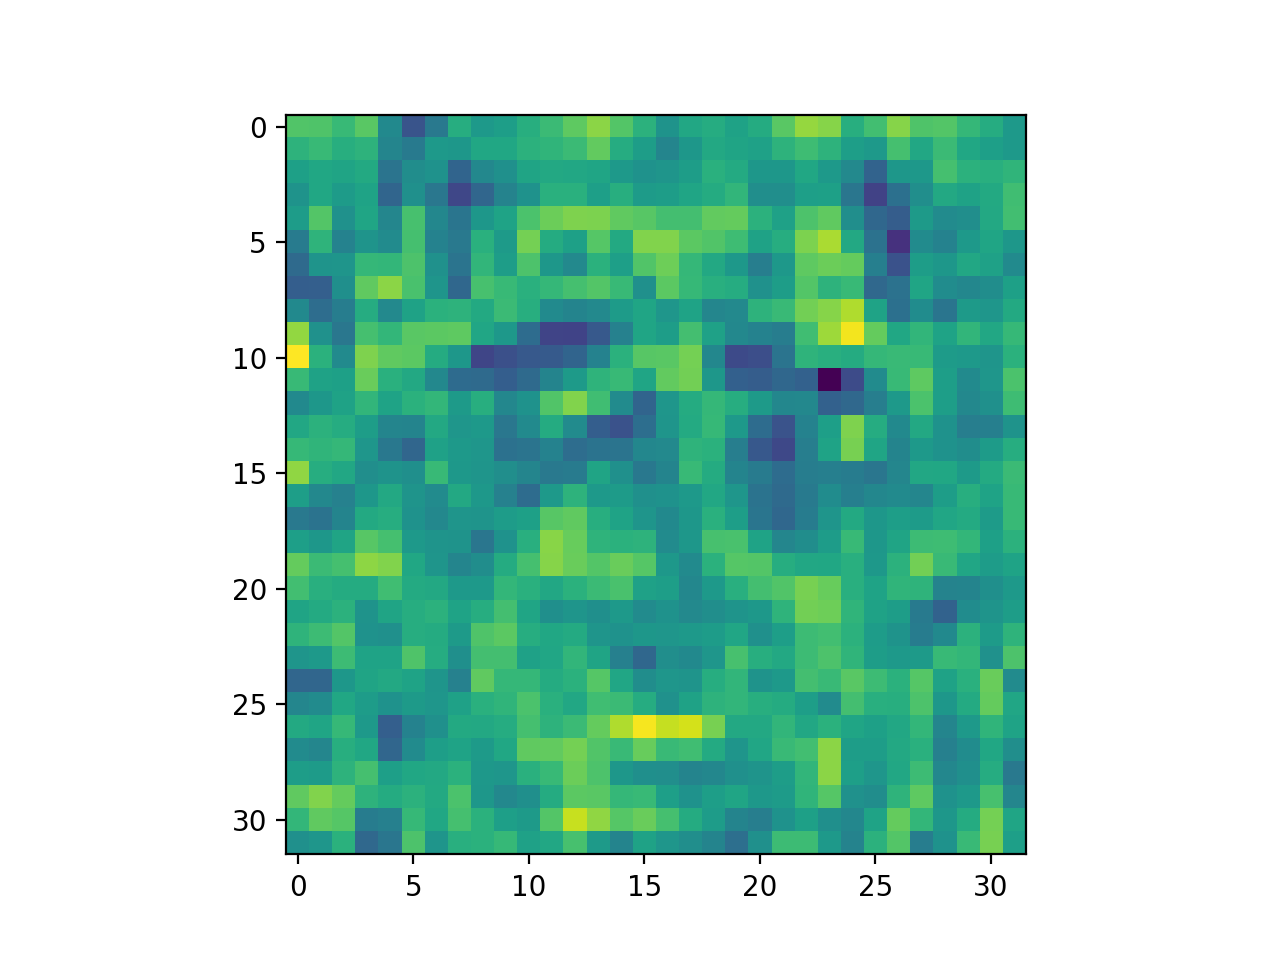
\includegraphics[width=.8\linewidth]{part4a1}
  \caption{$\theta$ got from full training set with larger $\alpha$}
  \label{fig:4b1}
\end{subfigure}%
\begin{subfigure}{.55\textwidth}
  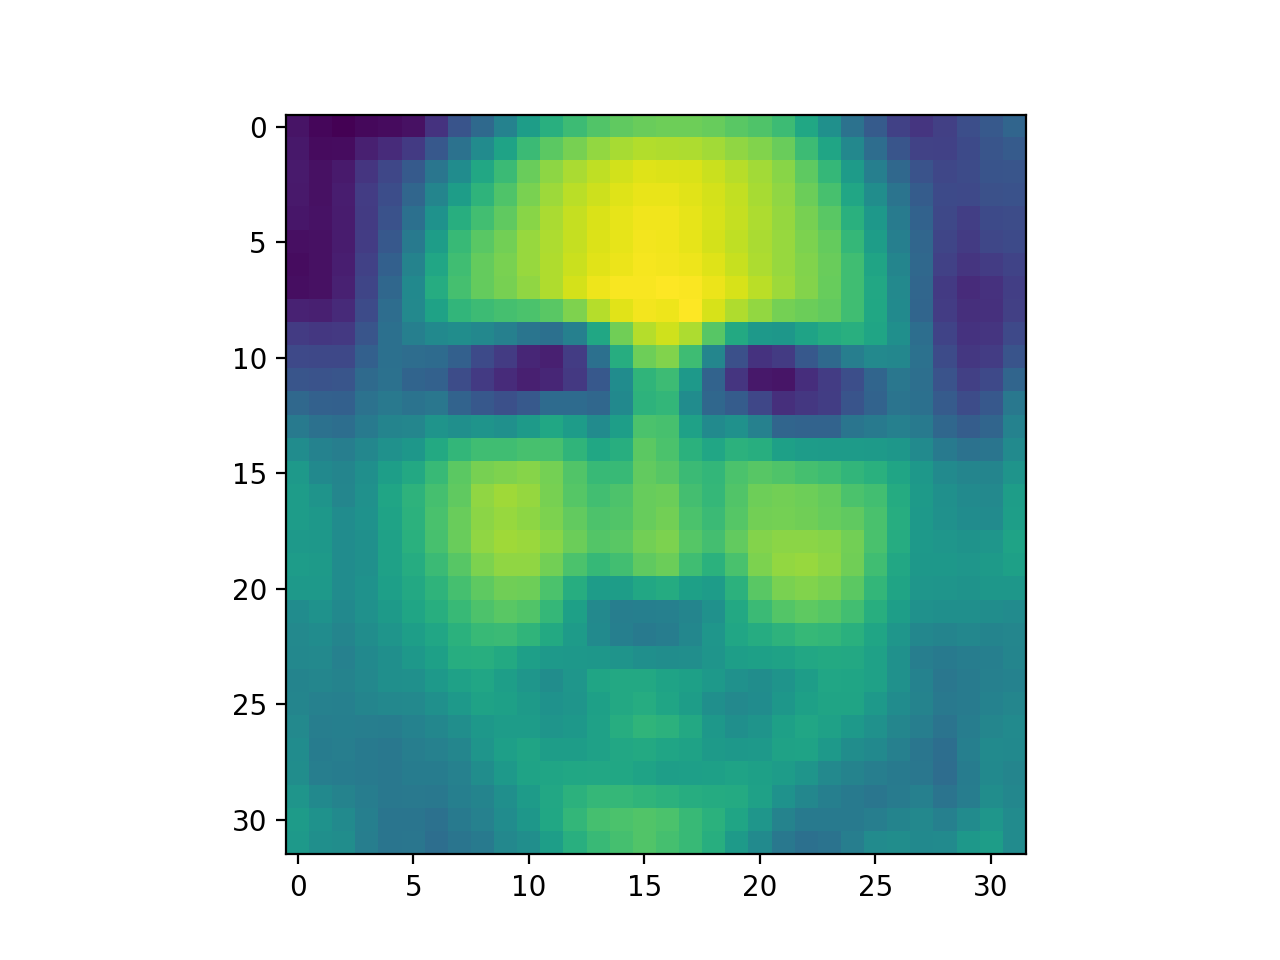
\includegraphics[width=.8\linewidth]{part4b.png}
  \caption{$\theta$ got from a full training set with smaller $\alpha$}
  \label{fig:4b2}
\end{subfigure}%

\caption{}
\label{fig:part4b}
\end{figure*}

Figure 4(b) looks similar to Figure 3(b). The faces are both obvious in them compare to Figure 4(a) and Figure 3(a). However, the two images are obtained by different methods. Figure 3(b) was computed by using a training set of size two, with one image from each actor. So the theta follows the face of the actor in the one image.\\
Figure 4(b) was obtained by using a full size training set. What I changed in code in order to get the image is $\alpha$. I made $\alpha$ really small which is $1e-14$. As mentioned in Part 3, when alpha is small enough, the gradient descent function diverges fast, so it won't be able to fit many images. Thus the theta will looks like the first few images processed.


\end{homeworkProblem}
\clearpage

%----------------------------------------------------------------------------------------
%	PROBLEM 5
%----------------------------------------------------------------------------------------

\begin{homeworkProblem}




\begin{table}[ht]
\centering
\begin{tabular}{lrrrrr}
  \hline
 & Size(training) & Size(validation) & Performance on Training set($\%$) & Performance on Validation Set($\%$) \\ 
  \hline
  & 70 & 10 & 100.0 & 93.3333333333  \\ 
  & 50 & 10 & 100.0 & 88.3333333333  \\ 
  & 30 & 10 & 100.0 & 83.3333333333  \\ 
  & 10 & 10 & 100.0 & 81.6666666667\\ 
   \hline
\end{tabular}
\end{table}

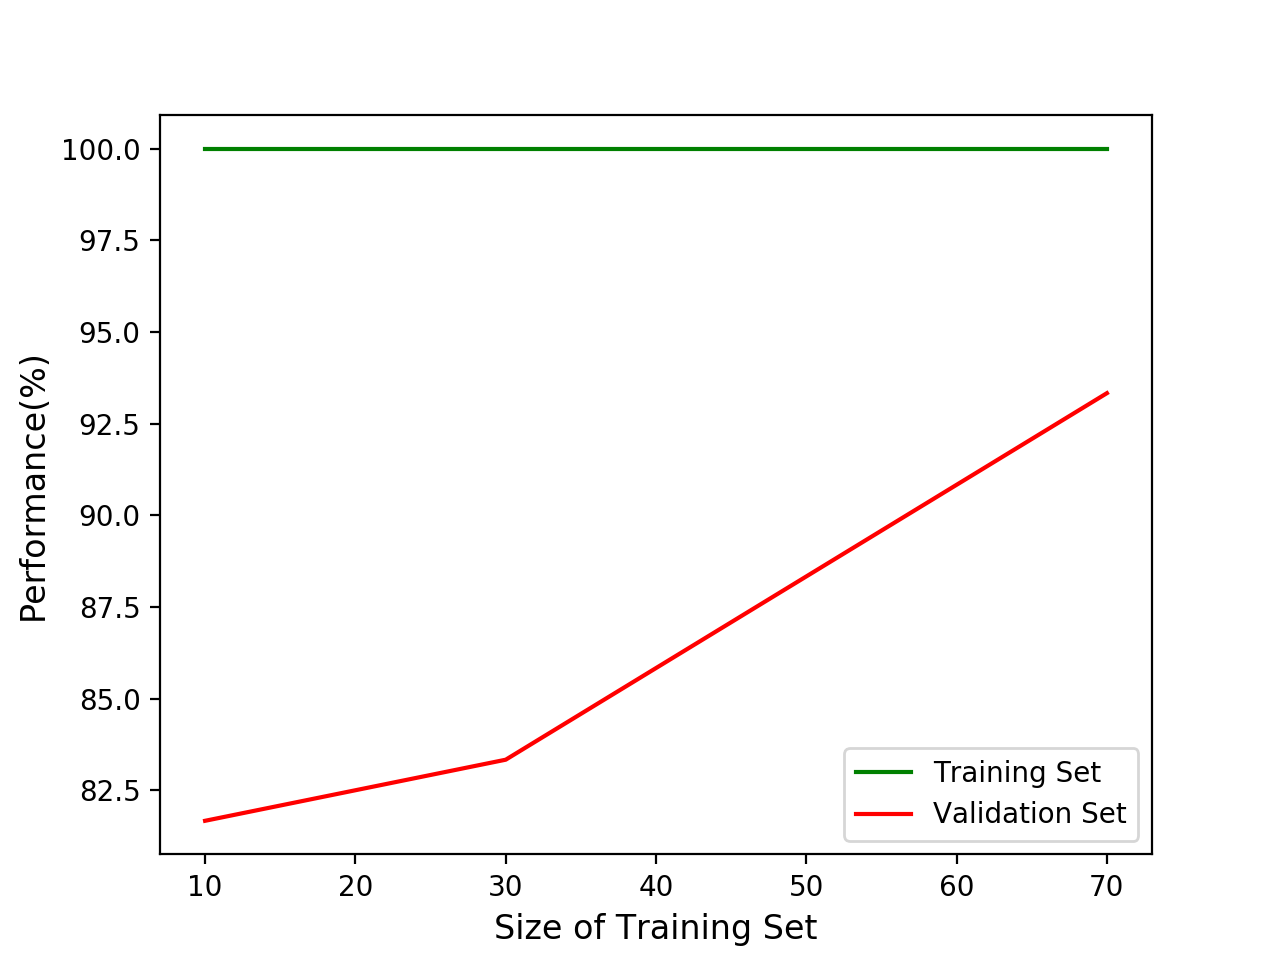
\includegraphics[scale = 0.7]{part5.png}\\

The above graph is the performance of the classifiers on the training and validation sets vs the size of the training set. The performance of the classifier on the training set is always $100\%$. However, the performance of the classifier on the validation set varies according to the size of the training set. As the size of the training set increases, the accuracy of the classifier on validation set also increases.\\

The accuracy of the classifier on test set of the six actors not included in act is $88.3333333333\%$.\\
The six actor and actresses are ['Gerard Butler', 'Michael Vartan', 'Daniel Radcliffe', 'Fran Drescher', 'America Ferrera', 'Kristin Chenoweth'].\\



\end{homeworkProblem}
\clearpage

%----------------------------------------------------------------------------------------
%	PROBLEM 6
%----------------------------------------------------------------------------------------

\begin{homeworkProblem}

a)\\

\[J(\boldsymbol\theta) = \sum_{i} \sum_{j} (\boldsymbol\theta_{i,j}^{T} \boldsymbol x_{ij} - \boldsymbol y_{ij})^2 \]
\[\frac{\partial J}{\partial \theta_{pq}} = \partial \boldsymbol\theta_q (2 \sum_{j} (\boldsymbol\theta_{p,j}^{T} \boldsymbol x_{pj} - \boldsymbol y_{pj}) \boldsymbol x_{pj})\]
\[ = 2(\theta_{p,q}^{T} x_{pq} - y_{pq}) x_{pq}\]

b)\\
\[\frac{\partial J}{\partial \boldsymbol \theta} = \sum_{i} \sum_{j} 2(\theta_{p,q}^{T} x_{pq} - y_{pq}) x_{pq}\]
\[ = 2 \sum_{i} (\boldsymbol\theta_{p}^{T} \boldsymbol x_{p} - \boldsymbol y_{p}) \boldsymbol x_{p}\]
\[ = 2 \boldsymbol X (\boldsymbol \theta^{T} \boldsymbol X - \boldsymbol Y)^T \]
The dimension of $\boldsymbol x$ is (1025, 240). $\boldsymbol x$ is a matrix containing all the input training data and additional 1's at the top of each column. Each column represents an image.\\
The dimension of $\boldsymbol \theta$ is (1025, 4). $\boldsymbol \theta$ is the parameter linear regression. It is computed by the gradient descent function. $\boldsymbol \theta_0$ is the intercept, others are parameters aligned with each pixel.\\
The dimension of $\boldsymbol y$ is (4, 280). $\boldsymbol y$ is the observed result. Each column represents the result of an image with the corresponding row be $1$. Other rows in that column are $0$. There are six actors and actresses, so the number of rows is 4. The number of columns is 280 since there are 280 images in the training set (70 images per actor, 4 actors in total).\\


c)\\
\includegraphics[scale = 0.7]{part6c.png}\\
The function $f\_part6$ is the implemented cost function and $df\_part6$ is the implemented vectorized gradient function.\\ 


d)\\
The following function is the code I used to compute the derivative of the finite-difference approximation.\\
x and y are defined randomly with the corresponding size. The theta is also defined randomly.\\
$theta\_h$ is a matrix of size (1025, 4) containing all zeros except one of the points is changed to $h$.\\
I have changed (0, 0) and (1, 2) of the $theta\_h$ to $h$, respectively.\\
\includegraphics[scale = 0.7]{part6d1.png}\\
The following is the result I got from the code above. We can see that for (0,0). The result of the finite-difference approximation is close to the (1, 1) of the result of the gradient function. And for (1, 2), the result of the finite-difference approximation is close to the (2, 3) of the result of the gradient function. Before I chose this h, I did the test among several coordinates and adjusted h to make sure the result from the finite-difference approximation is close to the corresponding result from the gradient function. Either the $h$ is too large or too small would make the finite-difference approximation not accurate enough.\\
\includegraphics[scale = 0.7]{part6d2.png}\\




\end{homeworkProblem}
\clearpage

%----------------------------------------------------------------------------------------
%	PROBLEM 7
%----------------------------------------------------------------------------------------

\begin{homeworkProblem}

The performances of the classifier on training set and validation are $92.1428571429\%$ and $85.0\%$, respectively. 

For gradient descent, the theta I choose is an array of zeros of size (1025, 6), the $\alpha$ I chose is $0.0000005$. \\
The parameters does make sense because the gradient descent function does converge and finds a minimum cost function. Moreover, the performances of the classifier on training set and validation set show that it was not overfitted.\\

Output values are assigned like this:

\begin{verbatim}
'bracco':  [1,0,0,0,0,0]
'gilpin':  [0,1,0,0,0,0]
'harmon':  [0,0,1,0,0,0]
'baldwin': [0,0,0,1,0,0]
'hader':   [0,0,0,0,1,0] 
'carell':  [0,0,0,0,0,1]
\end{verbatim}
The result I used to classify the image is $\boldsymbol \theta^T \boldsymbol x$, where $\theta$ is computed by the classifier and $x$ is the pixels of the image. More specifically, the result is computed by $[\theta_1^T x_i,  \theta_2^T x_i,  \theta_3^T x_i,  \theta_4^T x_i,  \theta_5^T x_i,  \theta_6^T x_i]$, since $1$ is added to $x$. Therefore, the result would be a matrix of size $(6, 1)$. As shown above, the six indexes would be correspond to each actor. The value of each row in the matrix corresponds to the similarity of the image to the actor. So if row i has the highest value among the six, that means the image is most similar to actor i.



\end{homeworkProblem}
\clearpage

%----------------------------------------------------------------------------------------
%	PROBLEM 8
%----------------------------------------------------------------------------------------

\begin{homeworkProblem}

\begin{figure*}[!ht]
\begin{subfigure}{.35\textwidth}
  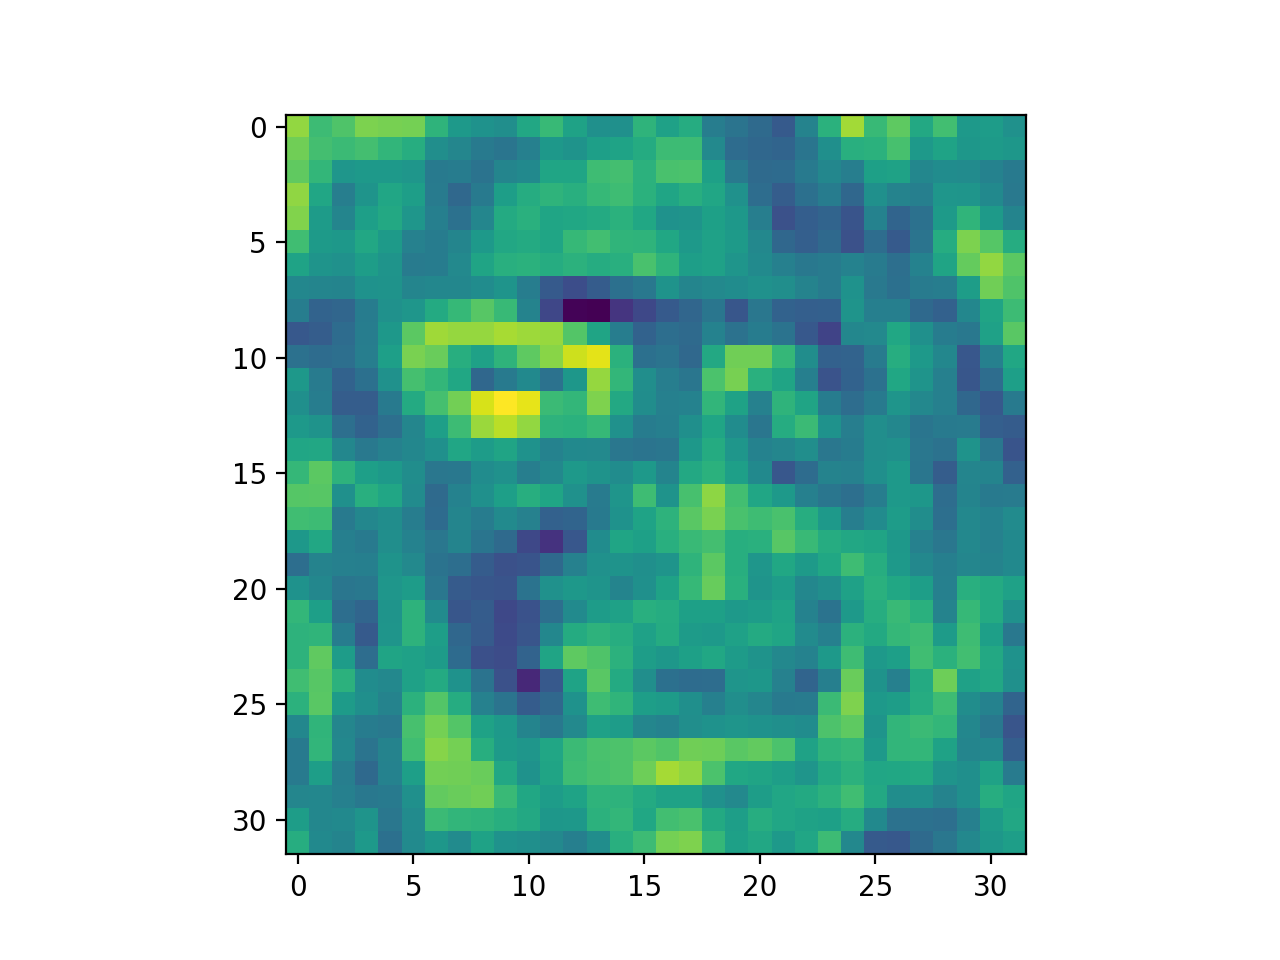
\includegraphics[width=1\linewidth]{bracco}
  \caption{Lorraine Bracco}
  \label{fig:8.1}
\end{subfigure}
\begin{subfigure}{.35\textwidth}
  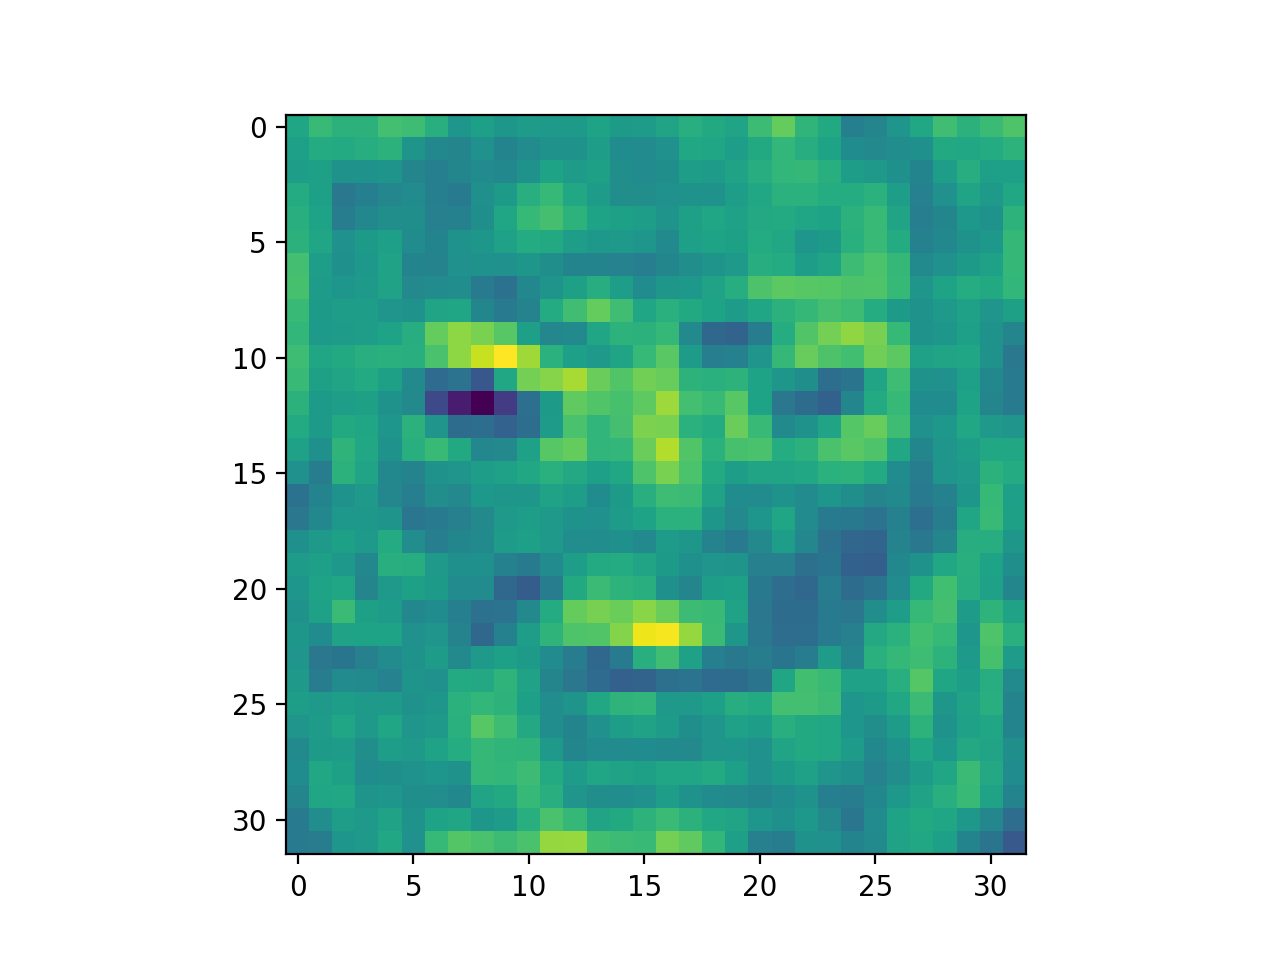
\includegraphics[width=1\linewidth]{gilpin}
  \caption{Peri Gilpin}
  \label{fig:8.2}
\end{subfigure}%
\begin{subfigure}{.35\textwidth}
  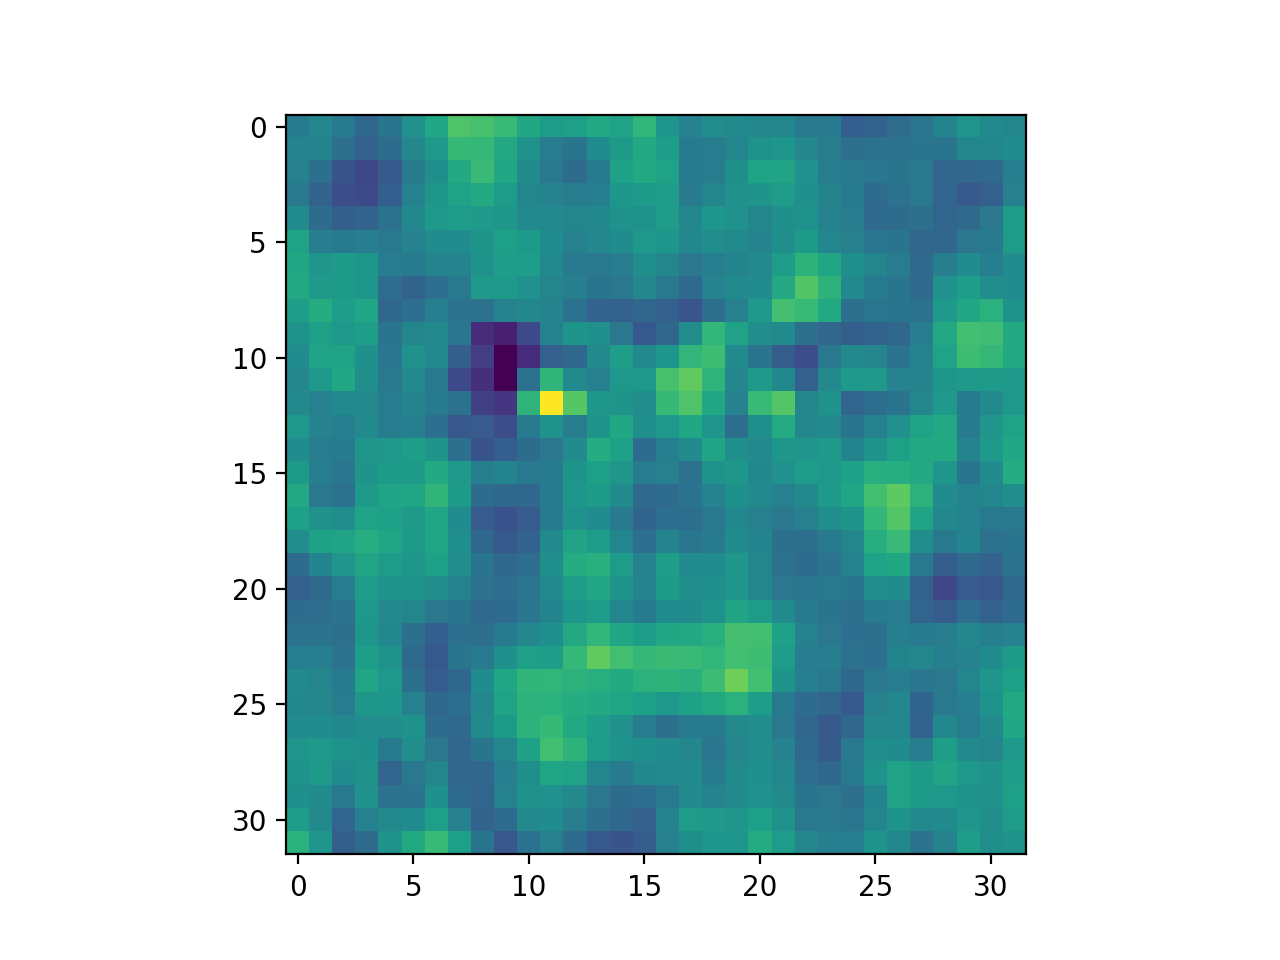
\includegraphics[width=1\linewidth]{harmon}
  \caption{Angie Harmon}
  \label{fig:8.3}
\end{subfigure}
\begin{subfigure}{.35\textwidth}
  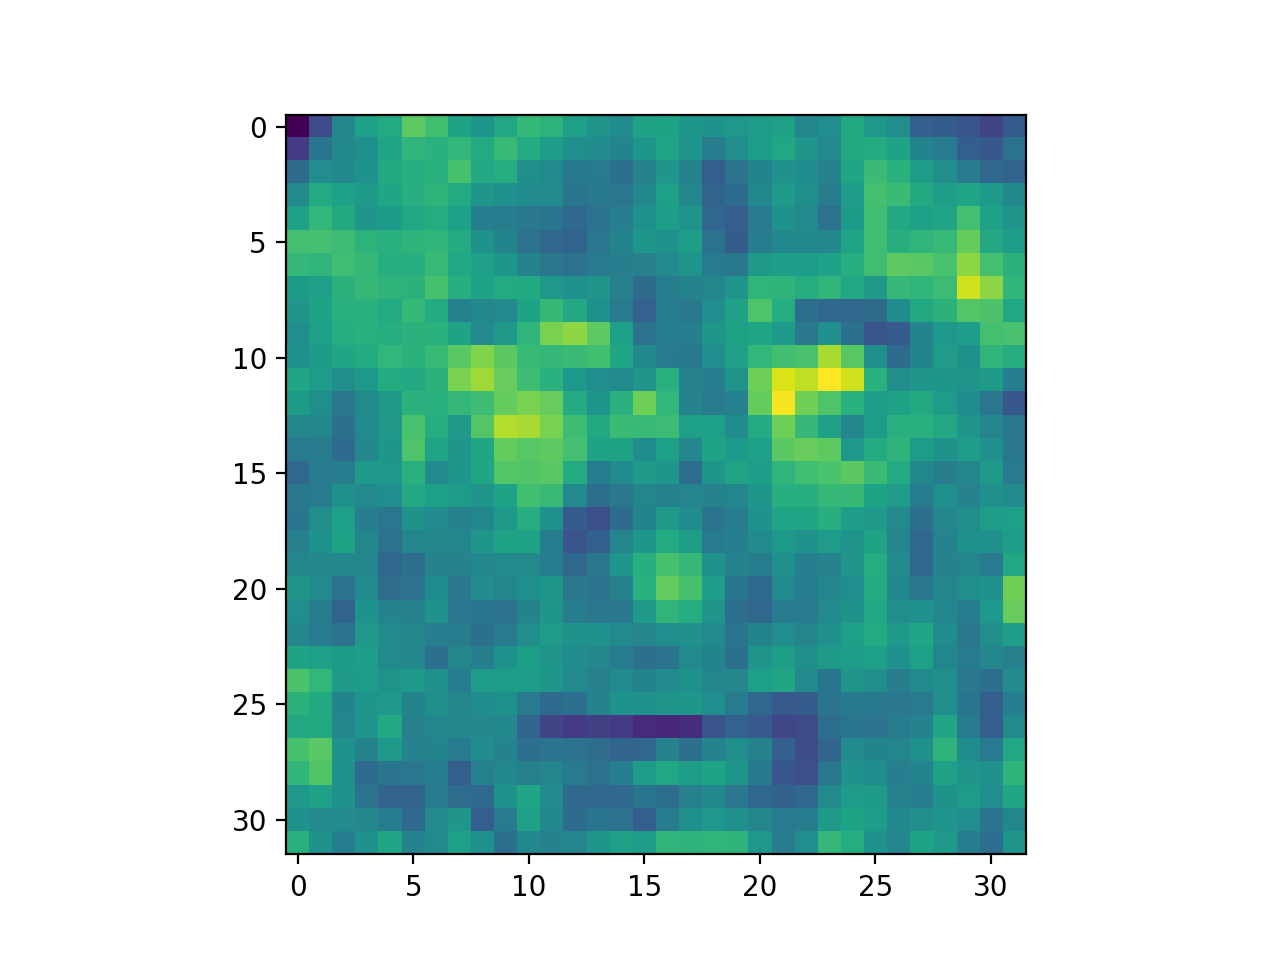
\includegraphics[width=1\linewidth]{baldwin}
  \caption{Alec Baldwin}
  \label{fig:8.4}
\end{subfigure}%
\begin{subfigure}{.35\textwidth}
  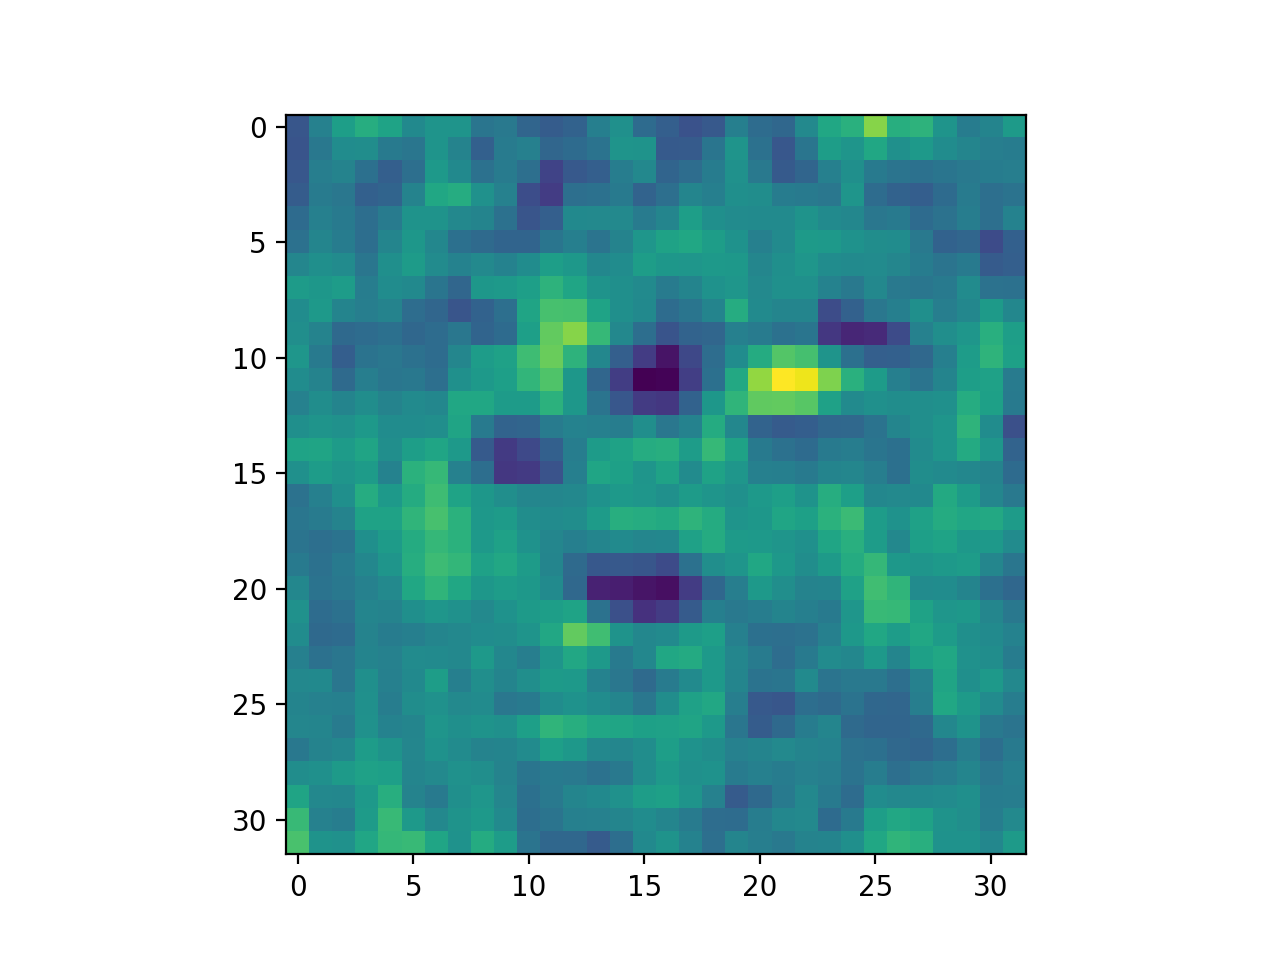
\includegraphics[width=1\linewidth]{hader}
  \caption{Bill Hader}
  \label{fig:8.5}
\end{subfigure}
\begin{subfigure}{.35\textwidth}
  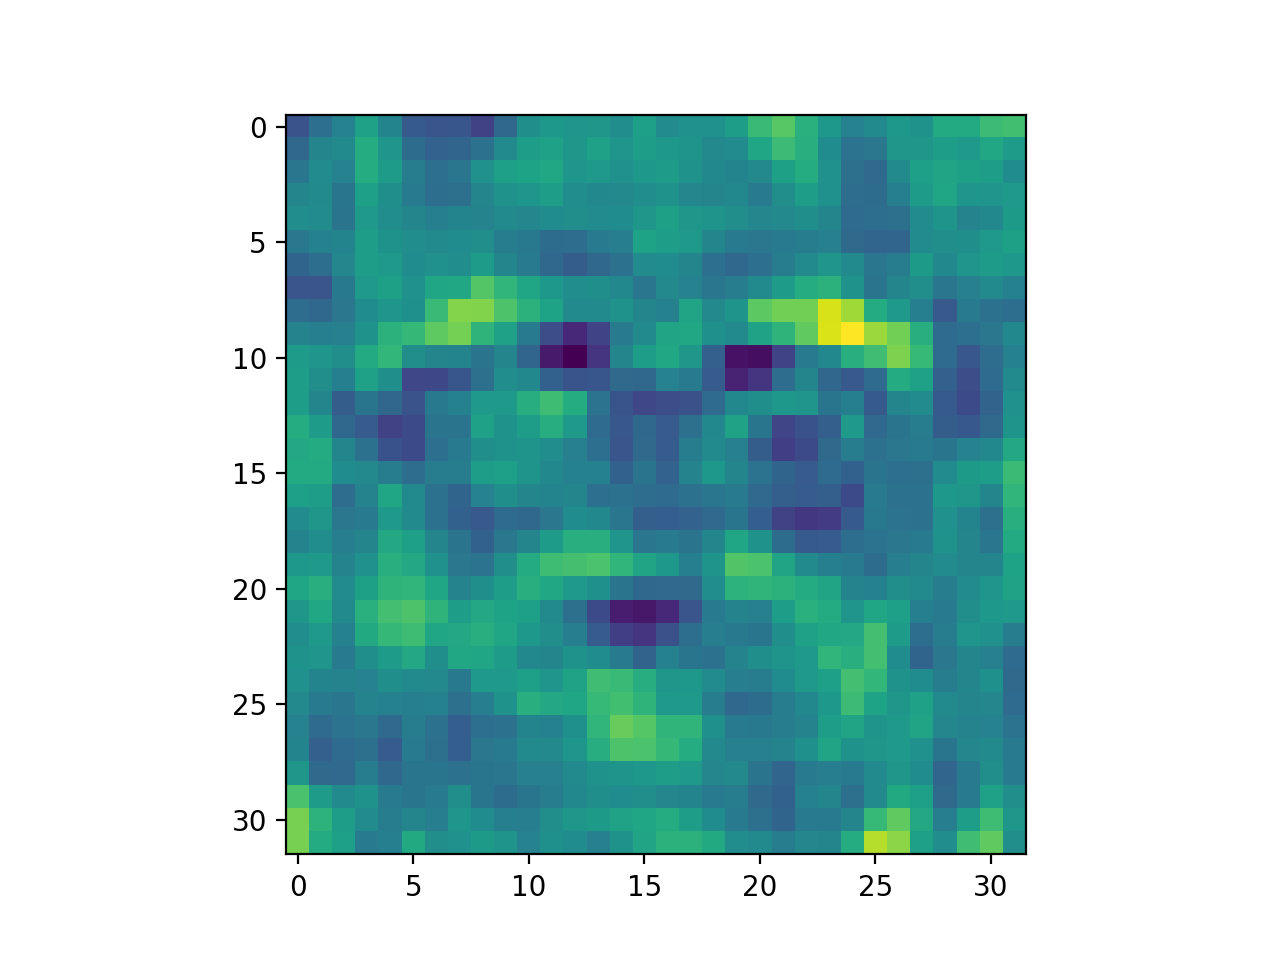
\includegraphics[width=1\linewidth]{carell}
  \caption{Steve Carell}
  \label{fig:8.6}%
\end{subfigure}
\caption{}
\label{fig:part8}
\end{figure*}





\end{homeworkProblem}
\clearpage

%----------------------------------------------------------------------------------------

\end{document}